% !TEX root = main.tex
% Appendix. A: formal setup. B: executors. C: Lemmas 1-2 and Theorem 1(ii).
% D: Theorem 2 (two-path). E: Theorem 1(i). F: Proposition 2 (routing). G: experiments. H: reproducibility.
% F: reproducibility.
\providecommand{\reg}[1]{\ensuremath{\mathsf{#1}}}

\section{Formal setup}
\label{app:formal}

This section states the definitions and assumptions that the main text summarizes.

\label{app:setup}
Throughout, $K=2$: counts are bits, and a logit vector $\bm z\in\R^K$ has two entries. We keep the vector notation because the
proofs use the softmax and cross-entropy of these logits; the scalar logit of the main text is $z=z_0-z_1$.

\begin{table}[H]
\centering\small
\caption{Notation of the main text. Constants $c,C>0$ depend only on the architecture constants of
\cref{ass:arch,ass:init} (namely $a_0$, $\embconst$, $\attconst$, $\ballradius$), never on $n$, $\varepsilon$ or $\lambda$.}
\label{tab:notation}
\begin{tabular}{@{}ll@{}}
\toprule
Symbol & Meaning\\
\midrule
$n$, $p$, $\lambda$ & number of letters; probability of the query letter; $\lambda=1-2p$\\
$s_t$, $S$, $C_t$ & running count after $t$ letters; $S=(-1)^{s_0}$; $C_t=(-1)^{b_t}$\\
$\bm\theta$, $\varepsilon$ & all parameters; initialization scale\\
$\Lout$, $\Lstep$ & outcome and teacher-forced step cross-entropy (\cref{def:losses})\\
$a$, $g$, $q$, $k$ & state readout, gate readout, query and key strengths (both theorems)\\
$h_\phi$ & averaging path of the two-path family (\cref{thm:matched} only)\\
\bottomrule
\end{tabular}
\end{table}

\begin{definition}[Counting]
\label{def:task}
A prompt has a start bit $s_0$, uniform on $\{0,1\}$, and letters $w_1,\ldots,w_n$ drawn i.i.d.\ from an alphabet
in which a fixed query letter $w^\star$ has probability $p\in(0,1/2)$. With $b_t=\mathbf 1[w_t=w^\star]$,
$s_t=s_0+b_1+\cdots+b_t\pmod 2$, and the answer is $y=s_n$.
\end{definition}

\begin{definition}[Contraction coefficient]
\label{def:lambda}
\begin{equation}
 \mixrate=\E\bigl[(-1)^{b_t}\bigr]=1-2p\in(0,1).
 \label{eq:lambda}
\end{equation}
\end{definition}

\begin{definition}[Credit]
\label{def:credit}
For a target signal $\bm\xi\in\R^K$ and logits $\bm z_{\bm\theta}\in\R^K$, let $\cred_{\bm\xi}(\bm\theta)=\E[\langle\bm z_{\bm\theta},\bm\xi\rangle]$.
The \emph{credit} for $\bm\xi$ is $\|\nabla_{\bm\theta}\cred_{\bm\xi}\|=\bigl\|\E\bigl[(\Jz)^\top\bm\xi\bigr]\bigr\|$.
For $\bm\xi=\bm y-\bm u$ we have $\langle\bm z,\bm y-\bm u\rangle=\frac12 z\,(-1)^{s_n}$, so this is half the scalar credit of \cref{sec:outcome}.
\end{definition}

\paragraph{Losses and credit.}

\begin{definition}[Outcome and step losses]
\label{def:losses}
Let $\bm z_t(\bm\theta)\in\R^K$ be the state logits at the position that predicts $s_t$, and $\bm z_{\bm\theta}$
those at the answer position. The \emph{outcome loss} is $\Lout(\bm\theta)=\E[-\log\softmax(\bm z_{\bm\theta})_y]$, and $\bm y=\bm e_y$ is the one-hot answer.
Write $\ell_t(\bm\theta)=\E[-\log\softmax(\bm z_t(\bm\theta))_{s_t}]$. The first state prediction is a boundary case: the previous
count $s_0$ sits in the prompt rather than at the predicting position. The \emph{step loss} is therefore the teacher-forced
transition loss
\[
 \Lstep(\bm\theta)=\frac{1}{n-1}\sum_{t=2}^n\ell_t(\bm\theta),
\]
and $\Lstep^{\mathrm{all}}(\bm\theta)=\tfrac{1}{n}\sum_{t=1}^n\ell_t(\bm\theta)$ also includes $t=1$.
\end{definition}

With $\bm u=K^{-1}\bm 1$, the outcome credit functional is $\outcredit=\cred_{\bm y-\bm u}$ (\cref{def:credit}). At zero
attention scores the network is additive over positions (\cref{prop:network}(iii)), so every interaction among letters passes through the
scores; the \emph{score-mediated credit} is the credit of the score-dependent part $\mathbf J_{\mathrm{score}}=\Jz-\mathbf J^{[0]}$ of the Jacobian (\cref{eq:score-split}),
$\bigl\|\E[\mathbf J_{\mathrm{score}}^\top(\bm y-\bm u)]\bigr\|$.

\paragraph{Architecture and initialization.}

\begin{assumption}[Architecture]
\label{ass:arch}
A causal Transformer with two blocks of softmax heads and ReLU MLPs, learned token and position
embeddings, no LayerNorm, any widths (residual $d_{\mathrm{res}}$, head $d_{\mathrm h}$, MLP $w$) and a linear readout $\mathbf V$;
every logit vector is $\bm z=\mathbf V\bm h$ with $\bm h$ independent of $\mathbf V$. A head may have a fixed, input-independent causal submask;
ordinary attention uses the full prefix.
\end{assumption}

\begin{assumption}[Initialization]
\label{ass:init}
\emph{Scale.} $\bm\theta_0=\initscale\tilde{\bm\theta}$ with $\initscale\le\initscale_0:=c\min(1,\frac{1}{N_b})$, where every weight matrix and embedding block of $\tilde{\bm\theta}$ has operator norm
at most $a_0$ and the value-token embeddings have smallest singular value at least $\embconst>0$.

\emph{Biases.} Every MLP bias satisfies $|\tilde b_m|\ge1$, and each MLP bias vector has norm at most $N_b$.

\emph{Neighbourhood.} We work on
$\initball=\{\bm\theta:\|\bm\theta-\bm\theta_0\|\le\ballradius\initscale\}$ with $\ballradius=\min(\frac{1}{8},\frac{\embconst}{4})$.
\end{assumption}

\begin{assumption}[Task]
\label{ass:task}
The task is binary counting with $0<p<1/2$ (\cref{def:task}), so $0<\mixrate<1$.
\end{assumption}

\paragraph{Constants and widths.} On $\initball$, no ReLU unit changes sign (\cref{app:network}). Constants $c,C>0$ depend only on $a_0$, $\embconst$, $K$
and the numbers of blocks and heads, never on the widths, $n$, $\initscale$ or the time. Fan-in-scaled initialization
satisfies \cref{ass:init} w.h.p.\ at every width, with $a_0$ bounded in terms of the largest block aspect ratio,
$\embconst\ge\tfrac{1}{2}$ and $N_b\le2\sqrt w$, provided the MLP biases are drawn with $|\tilde b_m|\in[1,2]$, which default
initializations (zero or small biases) do not do; at the executor width the aspect ratios are bounded, so the theorems
hold there with $n$-independent constants for $\initscale\le c\min(\mixrate,n^{-1/2})$ (\cref{rem:end-width}).

\paragraph{Parameters and training.}

\begin{assumption}[Training]
\label{ass:gd}
Full-batch gradient flow $\tfrac{d\bm\theta}{dt}=-\mathbf P\nabla_{\bm\theta}\mathcal L(\bm\theta)$ on $\Lout$ or $\Lstep$, where $\mathbf P$ is the orthogonal
projection onto a fixed set of trained parameter blocks; $\mathbf P=\mathbf I$ trains every parameter.
\end{assumption}

\label{rem:norms}Parameters carry the Euclidean norm of the vectorized parameters (Frobenius on each block).


\section{Exact two-block executors}
\label{app:architectures}

This section proves \cref{prop:represent}. An implementation of the construction is in the accompanying code repository.

\paragraph{Architecture.}
\label{app:construction}
\label{app:model}
Each block has three heads with $d_{\mathrm h}=2n+6$ (the number of positions) and one ReLU MLP of width $\max\{|\Sigma|,3K(n+1),2n+1\}$;
there is no LayerNorm:
\begin{align*}
 \bm h_i&\leftarrow \bm h_i+\sum_{h=1}^{3}\sum_{j\le i}\operatorname{softmax}_{j\le i}\Bigl(\tfrac{1}{\sqrt{d_{\mathrm h}}}(\mathbf W^{(h)}_Q\bm h_i)^{\!\top}\mathbf W^{(h)}_K\bm h_j\Bigr)\mathbf W^{(h)}_V\bm h_j,\\
 \bm h_i&\leftarrow \bm h_i+\mathbf W_{\mathrm{out}}\relu(\mathbf W_{\mathrm{in}}\bm h_i+\bm b_{\mathrm{in}}),\qquad \mathrm{logits}_i=\mathbf V\,\bm h_i .
\end{align*}

\paragraph{Registers.} The residual stream is the concatenation of one-hot registers
\[
 \underbrace{\reg{tl}}_{|\Sigma|}\ \underbrace{\reg{tv}}_{K}\ \underbrace{\reg{pos}}_{d_{\mathrm h}}\ \underbrace{\reg{qry}}_{|\Sigma|}\ \underbrace{\reg{match}}_{1}\
 \underbrace{\reg{prev}}_{K}\ \underbrace{\reg{mt}}_{1}\ \underbrace{\reg{cnt}}_{1}\ \underbrace{\reg{s0}}_{K}\ \underbrace{\reg{out}}_{K},
 \qquad d_{\mathrm{res}}=2|\Sigma|+4K+d_{\mathrm h}+3 .
\]
$\reg r[a]$ is coordinate $a$ of register $\reg r$, and $\mathbf E_{\reg a\leftarrow\reg b}$ copies $\reg b$ into $\reg a$.

\paragraph{Layout.} Token ids: letters $0,\ldots,|\Sigma|-1$, value $v\mapsto|\Sigma|+v$, then SEP, ``:'', EOS. Positions ($0$-indexed):
\[
\begin{array}{ll}
 \text{prompt} & s_0@0,\quad w^\star@1,\quad w_t@(1+t),\quad \mathrm{SEP}@(n+2)\\
 \text{step row} & s_t@(n+2+t),\quad ``{:}"@(2n+3),\quad s_n@(2n+4)\\
 \text{outcome row} & ``{:}"@(n+3),\quad s_n@(n+4)
\end{array}
\]
Position $i$ predicts the token at $i+1$: $n+1+t$ predicts $s_t$, and $n+3$ predicts $s_n$ in the outcome row.

\paragraph{Programs.} State arithmetic is modulo $K$.
\begin{center}\small
\fitwidth{\begin{tabular}{@{}lll@{}}
\toprule
 & step executor & outcome executor\\
\midrule
block 1, head 1 & \multicolumn{2}{l}{$\reg{qry}\leftarrow$ the query, at every letter}\\
block 1, MLP & \multicolumn{2}{l}{$\reg{match}\leftarrow b_t$}\\
block 2, head 1 & $\reg{prev}\leftarrow\widetilde s_{t-1}$ & $\reg{cnt}\leftarrow$ mean of $\reg{match}$ over the letters\\
block 2, head 2 & $\reg{mt}\leftarrow\reg{match}$ of letter $t$ & $\reg{s0}\leftarrow s_0$\\
block 2, head 3 & copy the last displayed count to the answer position & ---\\
block 2, MLP & $\reg{out}\leftarrow\mathrm{lookup}(\reg{prev},\reg{mt})$ & $\reg{out}\leftarrow\mathrm{lookup}(\reg{s0},\reg{cnt})$\\
\bottomrule
\end{tabular}}
\end{center}

\paragraph{Route and average.} Let $\Omega_n=\max\{16,3\log(8(n+3))\}$, $C_Q=\Omega_n\sqrt{d_{\mathrm h}}$, and let $\mathrm{src}(i)\subseteq\{0,\ldots,i\}$ be the source set
of position $i$ (a fallback $\{f\}$ where none is listed). Set
\begin{equation}
 \begin{gathered}
 (\mathbf W_K)_{j,\reg{pos}[j]}=1,\qquad (\mathbf W_Q)_{j,\reg{pos}[i]}=C_Q\ \ (j\in\mathrm{src}(i)),\\
 \tfrac{1}{\sqrt{d_{\mathrm h}}}(\mathbf W_Q\bm h_i)^\top \mathbf W_K\bm h_j=\Omega_n\,[j\in\mathrm{src}(i)] .
 \end{gathered}
 \label{eq:route}
\end{equation}
With $\mathbf W_V=\mathbf E_{\reg a\leftarrow\reg b}$, the head writes into $\reg a$ the average of $\reg b$ over $\mathrm{src}(i)$, up to the leak bounded below; $|\mathrm{src}(i)|=1$ is a
route and $|\mathrm{src}(i)|>1$ an average. A fallback $f>i$ gives uniform attention at a position with no supervised prediction.

\paragraph{Lookup.} For a count $s$ and a bit $b\in\{0,1\}$, use one unit per pair $(s',b')$ with
\[
 \mathrm{pre}_{s'b'}=[s=s']+[b=b']-\tfrac{3}{2}=\begin{cases}\tfrac{1}{2}&(s',b')=(s,b),\\\le-\tfrac{1}{2}&\text{otherwise},\end{cases}
\]
and output weights $2\bm e_{s'+b'}$:
\begin{equation}
 \textstyle\sum_{s',b'}2\,\bm e_{s'+b'}\relu(\mathrm{pre}_{s'b'})=\bm e_{s+b}.
 \label{eq:lookup}
\end{equation}

\subsection{Both programs are exact}
\label{app:exact}

\begin{proof}[Proof of \cref{prop:represent}]
\emph{Ideal routing} ($\Omega_n=\infty$). With $m=\sum_tb_t$ and $[m=a]=\relu(m-a+1)-2\relu(m-a)+\relu(m-a-1)$,
\begin{gather*}
 \reg{match}_{1+t}=2\textstyle\sum_{a\in\Sigma}\relu\bigl([w_t=a]+[w^\star=a]-\frac{3}{2}\bigr)=b_t,\\
 \reg{prev}_{n+1+t}=\bm e_{s_{t-1}},\qquad \reg{mt}_{n+1+t}=b_t,\qquad
 \reg{cnt}_{n+3}=n\cdot\tfrac{1}{n}\textstyle\sum_tb_t=m,\qquad \reg{s0}_{n+3}=\bm e_{s_0},\\
 \reg{out}_{n+1+t}=\sum_{j,\iota}\bm e_{j+\iota}\,2\relu\Bigl([s_{t-1}=j]+[b_t=\iota]-\frac{3}{2}\Bigr)=\bm e_{s_t},\\
 \reg{out}_{n+3}=\sum_{j,a}\bm e_{j+a}[s_0=j][m=a]=\bm e_{s_n}.
\end{gather*}
The test $[s_0=j]$ is applied by adding $(n+2)([s_0=j]-1)$ to each of the three pre-activations of $[m=a]$. The readout has weight $20$
on $\reg{out}$ for value tokens and weight $20$ on the relevant $\reg{pos}$ coordinates for ``:'' and EOS; all unused maps are zero.

\emph{Finite scores.} A row puts total weight at most $\omega^{\mathrm{leak}}_n$ outside its sources, where
\[
 \omega^{\mathrm{leak}}_n=(d_{\mathrm h}-1)e^{-\Omega_n}<\frac{2(n+3)}{(8(n+3))^3}=\frac{1}{256(n+3)^2}.
\]
Hence
\begin{gather*}
 |\reg{match}-b_t|\le2\omega^{\mathrm{leak}}_n,\qquad \|\reg{prev}-\bm e_{s_{t-1}}\|\le\omega^{\mathrm{leak}}_n,\qquad |\reg{mt}-b_t|\le3\omega^{\mathrm{leak}}_n,\\
 |\reg{cnt}-m|\le3n\,\omega^{\mathrm{leak}}_n,\qquad \|\reg{s0}-\bm e_{s_0}\|\le\omega^{\mathrm{leak}}_n .
\end{gather*}
At the step positions,
\[
 \mathrm{pre}_{s_t}\ge\tfrac{1}{2}-4\omega^{\mathrm{leak}}_n>0>\max_{a\ne s_t}\mathrm{pre}_a,\qquad \reg{out}_{s_t}\ge1-8\omega^{\mathrm{leak}}_n .
\]
At the answer position the errors add to $(4n+2)\omega^{\mathrm{leak}}_n<\frac{1}{192}$, and the three-ReLU test is $1$-Lipschitz, so
\[
 \reg{out}_{s_n}\ge1-(4n+2)\omega^{\mathrm{leak}}_n,\qquad \max_{a\ne s_n}\reg{out}_a\le(4n+2)\omega^{\mathrm{leak}}_n .
\]
With readout weight $20$ and $a^\star$ the gold token at a supervised position,
\[
 z_{a^\star}-\max_{a\ne a^\star}z_a\ge20\min\bigl\{1-8\omega^{\mathrm{leak}}_n,\ 1-2(4n+2)\omega^{\mathrm{leak}}_n\bigr\}>19 .
\]

\emph{Open neighbourhood.} Let $\mathcal P_n$ be the finite set of gold prefixes and supervised positions. By continuity there is
$r_{\mathrm{exec},n}>0$ with
\[
 \|\bm\theta-\bm\theta^\star\|<r_{\mathrm{exec},n}\implies\max_{P\in\mathcal P_n}\|\bm z_{\bm\theta}(P)-\bm z_{\bm\theta^\star}(P)\|_\infty<\tfrac{19}{2},
\]
so every greedy prediction is $a^\star$, and induction over the continuation gives the claim.
\end{proof}


\section{Proofs of \texorpdfstring{\cref{thm:main,thm:outcome-end}}{Lemma 1 and Theorem 1(ii)}}
\label{app:damping-proof}
\label{app:mainproofs}
\label{app:credit-proof}

The three proof blocks below establish contraction, network locality and the plateau.

\subsection{Contraction}
\label{app:C-fourier}
\label{app:assumptions}




(A1)--(A4) denote \cref{ass:arch,ass:init,ass:task,ass:gd}, and (A3$'$) a uniform start. Unless stated otherwise the query and the start
count are fixed. Constants $c,C$ depend only on $a_0,\embconst,K$ and the numbers of blocks and heads. Every bound stated on $\initball$ also
holds on $\initball'=\{\bm\theta:\|\bm\theta-\bm\theta_0\|\le2\ballradius\initscale\}$, whose relative radius is at most $\min(\frac{1}{4},\frac{\embconst}{2})$; there
$|b_m|\ge(1-2\ballradius)\initscale\ge\frac{3}{4}\initscale$ and $\sigma_{\min}(\mathbf E_{\mathrm{val}})\ge\frac{\initscale\embconst}{2}$. The only width-dependent threshold is $\initscale_0=c\min(1,\frac{1}{N_b})$.

\begin{lemma}[Gradient split]
\label{lem:gradient-split}
For every differentiable model, with $\outcredit(\bm\theta)=\E[\langle\bm z_{\bm\theta},\bm y-\bm u\rangle]$,
\[
 \nabla_{\bm\theta}\Lout=\underbrace{\E\bigl[(\Jz)^\top(\bm p-\bm u)\bigr]}_{\text{answer-independent}}-\underbrace{\nabla_{\bm\theta}\outcredit}_{\text{answer-dependent}},\qquad
 \nabla_{\bm\theta}\outcredit=\E\bigl[(\Jz)^\top(\bm y-\bm u)\bigr].
\]
\end{lemma}

\begin{proof}
The logit gradient of the cross-entropy is $\bm p-\bm e_y=(\bm p-\bm u)-(\bm y-\bm u)$.
\end{proof}

\paragraph{Contraction.}\label{app:contraction}\label{app:target-spectrum} Each letter sign $C_t=(-1)^{b_t}$ has mean
$\E[C_t]=1-2p=\mixrate$, and with the start bit fixed the signs are independent.

\paragraph{Proof of \cref{lem:binary-loss-mixture}.} Let $K=2$, $0<p<1/2$, $\ell(x)=\log(1+e^{-x})$, and let $f_\theta(S,C_n)$ be
any predictor of the start sign $S$ and the last letter $C_n$, with
$L_{\mathrm{step}}=\E\,\ell(SC_nf_\theta)$, $L_{\mathrm{out}}=\E\,\ell(S\prod_{j\le n}C_j\,f_\theta)$ and
$L_{\mathrm{sym}}=\frac12\E[\ell(f_\theta)+\ell(-f_\theta)]$.

The hidden product $\prod_{j<n}C_j$ is independent of $(S,C_n)$ and equals $\pm1$ with probability
$(1\pm\lambda^{n-1})/2$. Conditioning on it,
$L_{\mathrm{out}}=\frac{1+\lambda^{n-1}}2L_{\mathrm{step}}+\frac{1-\lambda^{n-1}}2\E\,\ell(-SC_nf_\theta)$.
The two signed losses sum to $2L_{\mathrm{sym}}$, which gives the identity. Differentiation commutes with these finite expectations.

The identity concerns this restricted predictor; a count-reading path is outside it, which is why
\cref{thm:matched} needs its own proof.

\begin{lemma}[Conditional contraction]
\label{lem:target-contraction}
Fix the start bit and the query, so that the letters are independent. Let $\bm\xi=\bm y-\bm u$, $A\subseteq[n]$ and
$\mathcal F_A=\sigma(w_t:t\in A)$. Then
\begin{equation}
 \E[\bm\xi\mid\mathcal F_A]=\tfrac12\,S\prod_{t\in A}C_t\;\mixrate^{n-|A|}\,(1,-1)^\top,
 \qquad \bigl\|\E[\bm\xi\mid\mathcal F_A]\bigr\|=\tfrac1{\sqrt2}\,\mixrate^{n-|A|}.
 \label{eq:horizon}
\end{equation}
Hence for every square-integrable $\mathcal F_A$-measurable matrix $\mathbf H$ with $K$ rows,
 $\bigl\|\E[\mathbf H^\top\bm\xi]\bigr\|\le\mixrate^{n-|A|}\,\|\mathbf H\|_{L^2},\qquad \|\mathbf H\|_{L^2}:=\bigl(\E\|\mathbf H\|_F^2\bigr)^{1/2}.$
The exponent is attained by $\mathbf H=\E[\bm\xi\mid\mathcal F_A]$, so it is sharp.
\end{lemma}

\begin{proof}
For $K=2$, $\bm\xi=\bm e_{s_n}-\frac12\one=\frac12(-1)^{s_n}(1,-1)^\top$ and $(-1)^{s_n}=S\prod_tC_t$. Independence replaces each sign outside $A$
by its mean $\mixrate$, which gives \cref{eq:horizon}. The matrix bound follows by the tower property and Cauchy--Schwarz:
$\|\E[\mathbf H^\top\bm\xi]\|=\|\E[\mathbf H^\top\E[\bm\xi\mid\mathcal F_A]]\|\le\|\mathbf H\|_{L^2}\,\mixrate^{n-|A|}$.
\end{proof}

\subsection{Transformer score expansion}
\label{app:model-spectrum}

The contraction estimate helps only if we can control how many letters a network term uses. Expanding the attention scores does
this without asking the entire output to depend on a small set: each term has its own set of letters, and terms with larger sets
are smaller near initialization.

\paragraph{Score expansion.} For $\zeta\in[0,1]$, let $\bm z(\zeta)$ be the network with every score $\psi_{il}$, in both blocks, replaced by
$\zeta\psi_{il}$. Then $\bm z(1)=\bm z_{\bm\theta}$, and for every integer $k_0\ge0$,
\begin{equation}
 \bm z_{\bm\theta}=\sum_{k=0}^{k_0}\bm z^{[k]}+\bm z_{\mathrm{rem}},\qquad
 \bm z^{[k]}=\frac{1}{k!}\frac{d^k\bm z}{d\zeta^k}(0),\qquad
 \bm z_{\mathrm{rem}}=\int_0^1\frac{(1-\zeta)^{k_0}}{k_0!}\frac{d^{k_0+1}\bm z}{d\zeta^{k_0+1}}(\zeta)\,d\zeta .
 \label{eq:score-split}
\end{equation}
$\mathbf J^{[k]}$ and $\mathbf J_{\mathrm{rem}}$ are the corresponding Jacobian terms. A term \emph{reads} the letters whose inputs it contains.

\begin{proposition}[Score count and letter support]
\label{prop:score-degree}
Fix the start state and the query. For $\bm\theta\in\initball$, $\Jz=\sum_{k=0}^{k_0}\mathbf J^{[k]}+\mathbf J_{\mathrm{rem}}$, and there is $\attconst$ such that:
\begin{enumerate}[label=(\roman*),leftmargin=*,itemsep=2pt,topsep=2pt]
\item $\mathbf J^{[0]}=\mathbf J^{[0]}_\emptyset+\sum_{t=1}^n\mathbf J^{[0]}_t$, where $\mathbf J^{[0]}_\emptyset$ reads no letter, $\mathbf J^{[0]}_t$ reads only $w_t$, $\sup\|\mathbf J^{[0]}_\emptyset\|_F\le C\initscale$ and
$\sum_t\sup\|\mathbf J^{[0]}_t\|_F\le C\initscale^2$;
\item for $k\ge1$, $\mathbf J^{[k]}=\sum_\nu\mathbf T_{k,\nu}$, where each $\mathbf T_{k,\nu}$ reads at most $2k+1$ letters and $\sum_\nu\sup\|\mathbf T_{k,\nu}\|_F\le C\initscale^2(\attconst\initscale^4)^k$;
\item $\sup\|\mathbf J_{\mathrm{rem}}\|_F\le C\initscale^2(\attconst\initscale^4)^{k_0+1}$.
\end{enumerate}
The same bounds hold for $\bm z^{[k]}$ and $\bm z_{\mathrm{rem}}$ with one more factor $\initscale$. Suprema are over inputs; constants do not depend on
$n$, $k$ or $k_0$.
\end{proposition}

$\attconst$ is fixed once, large enough for \cref{prop:score-degree,prop:network}; it depends only on $a_0$, $\embconst$ and $K$.

\label{app:network}

\begin{proposition}[Bounds for the score expansion]
\label{prop:network}
Assume (A1)--(A2). Uniformly on $\initball$, at every position and input, with $\bm x_i$ the token-plus-position vector,
all derivatives with respect to $s$ are evaluated at $s=0$ along $\bm\theta+sv$.
Let $\|F\|_{\mathrm{abs}}$ be the absolute sum of $F$ at $\zeta=0$: expand $F$ into monomials, products of
parameter blocks, inputs $\bm x_j$ and input-independent attention weights; bound each monomial by the product of the norm bounds of its
parameter factors on the ball, of $\sup\|\bm x_j\|$ for its inputs, and of its weights; and sum these bounds before any cancellation:
\begin{enumerate}[label=(\roman*),leftmargin=*,itemsep=3pt,topsep=4pt]
\item with input-independent offsets $\bm O^1=\bm o_1$, $\bm O^2=\bm o_1+\bm o_2$: $\bm h_i^\ell=\bm x_i+\bm O^\ell+O(\initscale^2)$, $|\psi_{il}|\le C\initscale^4$,
$\|\bm z_i\|\le C\initscale^2$, $\|\dd{\bm z_i}{s}\|\le C\initscale\|v\|$;
\item for $k\ge1$, $\zeta\in[0,1]$ and $\|v\|=1$,
\[
 \frac{1}{k!}\Bigl\|\frac{d^k\bm z_i}{d\zeta^k}\Bigr\|\le C\initscale^3(C_0\initscale^4)^k,\qquad
 \frac{1}{k!}\Bigl\|\dd{}{s}\left(\frac{\mathrm d^k\bm z_i}{\mathrm d\zeta^k}\right)\Bigr\|\le C\initscale^2(C_0\initscale^4)^k;
\]
the same holds for the absolute sums at $\zeta=0$, for $\bm h^2_i$ with one power of $\initscale$ fewer, and for the Taylor remainder with $k=k_0+1$;
\item the zero-score network is affine in the inputs; its transported logit terms have tangent $O(\initscale^2)$, and direct-input and
input-free terms have tangent $O(\initscale)$; an order-$k$ coefficient contains at most $2k+1$ inputs; a one-score logit term has size
$O(\initscale^7)$ and tangent $O(\initscale^6)$;
\end{enumerate}
The constants do not depend on $n$, the widths or $k$.
\end{proposition}

\begin{proof}
For a network quantity $F$ let $F^{[k]}(\zeta)=\frac{1}{k!}\frac{d^kF}{d\zeta^k}(\zeta)$, so that $\bm z^{[k]}=\bm z^{[k]}(0)$, and write $\|F^{[k]}\|$ for its supremum over
inputs, positions and $\zeta\in[0,1]$ (the $\ell_1$ norm for attention rows).

\emph{(i).} $|b_m|\ge\frac{3}{4}\initscale>C\initscale^2\ge|(\mathbf W_{\mathrm{in}}\bm h)_m|$, so one activation matrix $\mathbf D_{\mathrm{act}}$ serves every input and every $\zeta$, and
\[
 \begin{aligned}
 \bm h_i^\ell&=\mathbf M_\ell\bigl(\bm h_i^{\ell-1}+\bm a_i^\ell\bigr)+\bm o_\ell,\\
 \mathbf M_\ell&=\mathbf I+\mathbf W^\ell_{\mathrm{out}}\mathbf D_{\mathrm{act}}\mathbf W^\ell_{\mathrm{in}},\qquad
 \bm o_\ell=\mathbf W^\ell_{\mathrm{out}}\mathbf D_{\mathrm{act}}\bm b^\ell.
 \end{aligned}
\]
with $\bm a_i^\ell=\sum_{\mathrm{heads}}\sum_{j\le i}\omega_{ij}\mathbf W_V\bm h^{\ell-1}_j$ and $\omega_{i\cdot}=\softmax(\zeta\psi_{i\cdot})$. Then
 \[
\begin{gathered}
\|\mathbf M_\ell-\mathbf I\|\le C\initscale^2,\\ \|\bm o_\ell\|\le CN_b\initscale^2\le C\initscale,\\ \|\dd{\bm o_\ell}{s}\|\le(a_0+2N_b)\initscale\le C,
\end{gathered}
\] 
and $\|\omega_{i\cdot}\|_1=1$. Induction over the two blocks gives (i).

\emph{Softmax calculus.} Let $\omega=\softmax(s)$ and
$\E_\omega[f]=\sum_j\omega_jf_j$. For a direction $\bm\nu$,
\begin{align*}
 \left.\dd{}{t}\omega_j(s+t\bm\nu)\right|_{t=0}
 &=\omega_j(\nu_j-\E_\omega[\bm\nu]),\\
 \left.\dd{}{t}\E_{\omega(s+t\bm\nu)}[f]\right|_{t=0}
 &=\E_\omega[\bm\nu f]-\E_\omega[\bm\nu]\E_\omega[f].
\end{align*}
After $k$ derivatives, each term has at most $k+1$ differentiable factors
and contains each direction once. The absolute coefficient sums satisfy
$a_{k+1}\le2(k+1)a_k$, $a_0=1$. Summing against the probability weights gives
\begin{equation}
 \bigl\|D^k\omega(s)[\bm\nu_1,\ldots,\bm\nu_k]\bigr\|_1\le2^kk!\prod_a\|\bm\nu_a\|_\infty .
 \label{eq:softmax-avg}
\end{equation}
For the smooth finite-dimensional maps in the fixed-ReLU region, the
higher-order chain rule \citep[Theorem~2]{clark2013faa} yields
\[
 \frac{1}{j!}\|D^jF\|\le Ac^j,\quad \|h^{[k]}\|\le ab^k
 \quad\Longrightarrow\quad
 \|(F\circ h)^{[k]}\|\le Aca\,b^k(1+ca)^{k-1},\quad k\ge1.
\]
Here the inner map's derivative bounds hold for every positive order; the
composition count is $\binom{k-1}{j-1}$.

\emph{(ii), values.} With $\|\bm\omega^{\ell,[0]}\|_1=1$, $\|\bm h^{0,[k]}\|=0$ for $k\ge1$, and $a_r\ge1$ in the compositions,
\begin{alignat*}{2}
 \|\psi^{\ell,[k]}\|&\le C\initscale^2\textstyle\sum_{a+b=k}\|\bm h^{\ell-1,[a]}\|\,\|\bm h^{\ell-1,[b]}\| &\qquad& \why{score is a product}\\
 \|(\zeta\psi^\ell)^{[k]}\|&\le\|\psi^{\ell,[k]}\|+\|\psi^{\ell,[k-1]}\| && \why{$(\zeta\psi)^{[k]}=\zeta\psi^{[k]}+\psi^{[k-1]}$}\\
 \|\bm\omega^{\ell,[k]}\|_1&\le\textstyle\sum_{j=1}^k2^j\sum_{a_1+\cdots+a_j=k}\prod_r\|(\zeta\psi^\ell)^{[a_r]}\| && \why{composition, \cref{eq:softmax-avg}}\\
 \|\bm a^{\ell,[k]}\|&\le C\initscale\textstyle\sum_{a+c=k}\|\bm\omega^{\ell,[a]}\|_1\,\|\bm h^{\ell-1,[c]}\| && \why{head output is a product}\\
 \|\bm h^{\ell,[k]}\|&\le C\bigl(\|\bm h^{\ell-1,[k]}\|+\|\bm a^{\ell,[k]}\|\bigr) && \why{affine block}\\
 \|\bm z^{[k]}\|&\le C\initscale\,\|\bm h^{2,[k]}\| && \why{readout}
\end{alignat*}
With $b=C\initscale^4$, block $1$ gives, for $k\ge1$, $\|\bm\omega^{1,[k]}\|_1\le b^k$ and $\|\bm a^{1,[k]}\|+\|\bm h^{1,[k]}\|\le C\initscale^2b^k$ (while $\|\bm h^{1,[0]}\|\le C\initscale$). Then $\|\psi^{2,[0]}\|\le C\initscale^4$,
$\|\psi^{2,[k]}\|\le C\initscale^5(k+1)b^k$ for $k\ge1$, and $\|(\zeta\psi^2)^{[k]}\|\le C(2b)^k$, so
\begin{gather*}
 \|\bm\omega^{2,[k]}\|_1\le C\sum_{j=1}^k\binom{k-1}{j-1}C^j(2b)^k\le C(Cb)^k,\\
 \|\bm a^{2,[k]}\|+\|\bm h^{2,[k]}\|\le C\initscale^2(Cb)^k,\qquad \|\bm z^{[k]}\|\le C\initscale^3(C_0\initscale^4)^k .
\end{gather*}

\emph{(ii), tangents, remainders, absolute sums.} Differentiating along $v$ replaces one factor of each product by its tangent, or one
$(\zeta\psi)^{[a]}$ in a softmax term, or adds $D^{j+1}\omega[\dd{(\zeta\psi)^{[0]}}{s},\ldots]$. With $\|\dd{\bm h^{0,[0]}}{s}\|=O(1)$, $\|\dd{\psi^{\ell,[0]}}{s}\|=O(\initscale^3)$
and $j+1\le2^k$ absorbed into $C_0^k$,
\begin{gather*}
 \|\dd{\bm\omega^{\ell,[k]}}{s}\|_1\le C\initscale^{-1}(C_0\initscale^4)^k,\qquad \|\dd{\bm a^{\ell,[k]}}{s}\|+\|\dd{\bm h^{\ell,[k]}}{s}\|\le C\initscale(C_0\initscale^4)^k,\\
 \|\dd{\bm z^{[k]}}{s}\|\le C\initscale^2(C_0\initscale^4)^k .
\end{gather*}
The integral remainder is bounded by the supremum of the next normalized derivative.

\emph{Absolute sums.} $\|\cdot\|_{\mathrm{abs}}$ is subadditive and submultiplicative, and $\|F\|\le\|F\|_{\mathrm{abs}}$. At $\zeta=0$ every attention row is an
input-independent probability vector $\bm\pi$ (uniform over the visible sites), and
 $\Bigl\|\textstyle\sum_j\pi_j\prod_rF_r(j)\Bigr\|_{\mathrm{abs}}\le\prod_r\max_j\|F_r(j)\|_{\mathrm{abs}} .$ 
At $\zeta=0$, $D^j\omega$ expands as $\omega(0)$-weights times products of direction entries and $\omega(0)$-averages, with total coefficient at most $2^jj!$,
so \cref{eq:softmax-avg} holds for absolute sums with $\|\bm\nu_a\|_\infty$ replaced by $\max_l\|\nu_{a,l}\|_{\mathrm{abs}}$. Hence every line of the recursion
above holds verbatim for $\|\cdot\|_{\mathrm{abs}}$ at $\zeta=0$, which gives the absolute-sum bounds of (ii).

\emph{Tangents of absolute sums.} Take the norm bound of every parameter factor at least $\initscale$ (weights and embeddings $(a_0+1)\initscale$,
biases $(N_b+1)\initscale$). An order-$k$ monomial has at most $C(k+1)$ factors: at most $k$ scores, each with $\mathbf W_Q$ and $\mathbf W_K$, and at
most $2k+1$ inputs, each carried by at most four parameter blocks. Replacing one factor by its unit-direction tangent multiplies the bound by at
most $\frac{1}{\initscale}$, so the tangent bound is at most $\frac{C(k+1)}{\initscale}\le\frac{C2^k}{\initscale}$ times the monomial bound, uniformly in the unit direction
$v$; this lets $\sup_v$ pass inside the sum over monomials.

\emph{(iii).} At zero scores the network is affine in the inputs (for a head with a submask, $\frac{1}{m_j}$ becomes one over the size of its
visible set):
\begin{gather*}
 \bm h^1_j=\mathbf M_1\Bigl(\bm x_j+\frac{1}{m_j}\sum_{l\le j}\mathbf W^1_V\bm x_l\Bigr)+\bm o_1,\\
 \bm z^{[0]}_i=\mathbf V\Bigl[\mathbf M_2\Bigl(\bm h^1_i+\frac{1}{m_i}\sum_{j\le i}\mathbf W^2_V\bm h^1_j\Bigr)+\bm o_2\Bigr].
\end{gather*}
Transported terms contain $\mathbf V$, $\mathbf W_V$ and some $\bm x_j$, so their tangent is $O(\initscale^2)$; direct-input and input-free terms have tangent $O(\initscale)$.
With $d(F)$ the number of input occurrences in $F$,
\begin{alignat*}{2}
 d(\bm h^{\ell,[a]})&\le2a+1 &\qquad& \why{induction on $\ell$}\\
 d(\psi^{\ell,[b]})&\le2b+2 && \why{score is a product of two residuals}\\
 d\bigl((\zeta\psi)^{[a]}\bigr)&\le2a && \why{$(\zeta\psi)^{[a]}=\psi^{[a-1]}$}\\
 d(\text{order-$k$ head term})&\le2a_1+\cdots+2a_j+2c+1=2k+1 && \why{$a_1+\cdots+a_j+c=k$}
\end{alignat*}
and affine MLPs and parameter derivatives add none. The one-score correction is
 $\frac{1}{m_i}\sum_{j\le i}\bigl(\psi_{ij}(0)-\bar\psi_i(0)\bigr)\mathbf W_V\bm h_j(0),\qquad \bar\psi_i(0)=\frac{1}{m_i}\sum_{l\le i}\psi_{il}(0);$ 
its logit terms contain $\mathbf V,\mathbf W_V,\mathbf W_Q,\mathbf W_K$ and three residual inputs, so they have size $O(\initscale^7)$ and tangent $O(\initscale^6)$.

\end{proof}

\begin{proof}[Proof of \cref{prop:score-degree}]
Expand each coefficient into monomials in parameters and inputs. A Jacobian entry of a monomial is a monomial with the same inputs, and the
Frobenius norm of a map into $\R^K$ is at most $\sqrt K$ times its operator norm.

\noindent(i) At zero scores the network is affine in the inputs (\cref{prop:network}(iii)): each term contains at most one input. Group the terms by
that input. At the answer position the direct input is fixed and contains no letter; the transported terms have tangent $O(\initscale^2)$, and
their coefficients sum absolutely to a constant because every zero-score attention row is a probability vector.

\noindent(ii) By \cref{prop:network}(iii) an order-$k$ monomial contains at most $2k+1$ inputs, and by \cref{prop:network}(ii) the absolute sum of the
tangents at $\zeta=0$ is at most $C\initscale^2(C_0\initscale^4)^k$; take $\attconst\ge C_0$.

\noindent(iii) Apply \cref{prop:network}(ii) with $k=k_0+1$. Logit bounds carry one more factor $\initscale$ than Jacobian bounds.
\end{proof}

\subsection{Exponential outcome plateau}
\label{app:thm1}

Combining \cref{lem:target-contraction,prop:network} gives the following credit bound.

\begin{lemma}[Credit summation]
\label{lem:score-sum}
Assume (A1)--(A3), $\bm\theta\in\initball$, $0<\initscale\le\initscale_0$ and $0<\mixrate<1$, with the start state and query fixed. Let
$k_0=\lceil\frac{n-1}{2}\rceil$. If $\attconst\initscale^4\le\frac{1}{2}\mixrate^2$, then
 $\bigl\|\E\bigl[\mathbf J_{\mathrm{score}}^\top(\bm y-\bm u)\bigr]\bigr\|\le C\initscale^6\mixrate^{n-3},\qquad \mathbf J_{\mathrm{score}}=\Jz-\mathbf J^{[0]}.$ 
If moreover $\initscale\le\mixrate$, then
\begin{equation}
 \|\nabla_{\bm\theta}\outcredit(\bm\theta)\|\le C\initscale\mixrate^n,\qquad |\outcredit(\bm\theta)|\le C\initscale^2\mixrate^n.
 \label{eq:thm1-full}
\end{equation}
The bounds persist after averaging over the start state and query.
\end{lemma}

\begin{proof}
Apply \cref{lem:target-contraction} to each term of \cref{prop:score-degree}, with $\|\mathbf H\|_{L^2}\le\sup\|\mathbf H\|_F$ and $\|\bm y-\bm u\|\le1$ for the remainder:
\begin{alignat*}{2}
 \bigl\|\E\bigl[(\mathbf J^{[0]})^\top(\bm y-\bm u)\bigr]\bigr\|&\le C\initscale\mixrate^n+C\initscale^2\mixrate^{n-1} &\qquad& \why{(i): $0$ or $1$ letter}\\
 \bigl\|\E\bigl[(\mathbf J^{[k]})^\top(\bm y-\bm u)\bigr]\bigr\|&\le C\initscale^2(\attconst\initscale^4)^k\mixrate^{n-2k-1} && \why{(ii): $\le2k+1$ letters, $k\ge1$}\\
 &=C\initscale^6\mixrate^{n-3}\Bigl(\frac{\attconst\initscale^4}{\mixrate^2}\Bigr)^{k-1} && \\
 \bigl\|\E\bigl[\mathbf J_{\mathrm{rem}}^\top(\bm y-\bm u)\bigr]\bigr\|&\le C\initscale^2(\attconst\initscale^4)^{k_0+1} && \why{(iii)}\\
 &=C\attconst\initscale^6\mixrate^{2k_0}\Bigl(\frac{\attconst\initscale^4}{\mixrate^2}\Bigr)^{k_0} && \\
 &\le C\initscale^6\mixrate^{n-3}\Bigl(\frac{\attconst\initscale^4}{\mixrate^2}\Bigr)^{k_0} && \why{$2k_0\ge n-1$}
\end{alignat*}
If $2k+1>n$, the factor $\mixrate^{n-2k-1}\ge1$ still bounds the credit. Since $\frac{\attconst\initscale^4}{\mixrate^2}\le\frac{1}{2}$, the
score-dependent terms sum to at most $3C\initscale^6\mixrate^{n-3}$, which is the first bound. Adding the zero-order term,
\begin{align*}
 \|\nabla_{\bm\theta}\outcredit\|&\le C\bigl(\initscale\mixrate^n+\initscale^2\mixrate^{n-1}+\initscale^6\mixrate^{n-3}\bigr),\\
 |\outcredit|&\le C\bigl(\initscale^2\mixrate^n+\initscale^3\mixrate^{n-1}+\initscale^7\mixrate^{n-3}\bigr),
\end{align*}
by \cref{lem:gradient-split} and the same argument for the logits, and $\initscale\le\mixrate$ reduces both to \cref{eq:thm1-full}.
\end{proof}

For $c$ small enough, $\initscale\le c\mixrate$ implies $\initscale\le\mixrate$ and $\attconst\initscale^4\le\frac{1}{2}\mixrate^2$, and $\initscale^2\le c\mixrate$ implies $\attconst\initscale^4\le\frac{1}{2}\mixrate^2$.

\begin{proof}[Proof of \cref{thm:main}]
Part (i) is \cref{lem:target-contraction}. For (ii), take $c\le(2\attconst)^{-1/2}$:
 $\initscale^2\le c\mixrate\implies \attconst\initscale^4\le\attconst c^2\mixrate^2\le\tfrac{1}{2}\mixrate^2,$ 
and \cref{lem:score-sum} gives both bounds.
\end{proof}

\begin{lemma}[Smoothness near initialization]
\label{lem:end-smooth}
Assume (A1)--(A2), $\initscale\le\initscale_0$. There is $C_1$, independent of $n$, $\initscale$ and the widths, such that for every $\bm\theta\in\initball'$ and
every unit direction $\bm v$,
 $\|\nabla_{\bm\theta}\Lout(\bm\theta)\|\le C_1\initscale,\qquad \Bigl|\frac{d^2}{ds^2}\Lout(\bm\theta+s\bm v)\big|_{s=0}\Bigr|\le C_1 .$ 
\end{lemma}

\begin{proof}
Along $\bm\theta+s\bm v$ at $s=0$, applying the product rule twice to the
two blocks and \cref{eq:softmax-avg} with $k=1,2$ gives
\[
 \|\bm z\|\le C\initscale^2,\qquad
 \left\|\dd{\bm z}{s}\right\|\le C\initscale,\qquad
 \left\|\frac{\mathrm d^2\bm z}{\mathrm d s^2}\right\|\le C.
\]
The ReLU pattern is fixed by \cref{prop:network}(i). These bounds use only
operator norms and attention-row $\ell_1$ norms bounded by one, so $C$ is
independent of $n$ and the widths.
For cross-entropy, the log-sum-exp derivative formula
\citep[Section~3.1.5]{boyd2004convex} gives
\[
 \nabla_{\bm z}\ell=\bm p-\bm e_y,\qquad
 \nabla_{\bm z}^2\ell=\operatorname{diag}\bm p-\bm p\bm p^\top,
 \qquad \|\nabla_{\bm z}\ell\|\le\sqrt2,\quad
 \|\nabla_{\bm z}^2\ell\|\le1.
\]
The chain rule therefore yields
$|\dd{\ell}{s}|\le C\initscale$ and
$|\mathrm d^2\ell/\mathrm d s^2|\le C$.
Average over prompts and take the supremum over unit $\bm v$.
\end{proof}

\paragraph{Outcome plateau.}\label{app:end} For one prompt, $\KL(\bm u\|\bm p)=\log\sum_ae^{z_a}-\log K-\langle\bm u,\bm z\rangle$, hence
\begin{equation}
 \Lout(\bm\theta)=\log K+\E\bigl[\KL(\bm u\,\|\,\bm p_{\bm\theta})\bigr]-\outcredit(\bm\theta).
 \label{eq:lo-identity}
\end{equation}

\begin{proof}[Proof of \cref{thm:outcome-end}]
\emph{Loss floor.} Let $B_n=C_2\initscale^2\mixrate^n$, with $C_2$ the constant $C$ of \cref{eq:thm1-full}, $\initscale\le c\mixrate$ and $\bm\theta\in\initball$.
\begin{alignat}{2}
 \Lout(\bm\theta)&=\log K+\E\,\KL(\bm u\,\|\,\bm p_{\bm\theta})-\outcredit(\bm\theta) &\qquad& \why{\cref{eq:lo-identity}}\nonumber\\
 &\ge\log K-B_n && \why{$\KL\ge0$, \cref{lem:score-sum}}\label{eq:lo-floor}
\end{alignat}

\emph{Escape time.} By \cref{lem:end-smooth}, $\Lout$ is smooth on $\initball$, so the flow is defined there. Let
$T_{\mathrm{exit}}=\inf\{t:\|\bm\theta(t)-\bm\theta_0\|>\ballradius\initscale\}$. For $t\le T_{\mathrm{exit}}$,
\begin{alignat*}{2}
 \ddt{\Lout}&=-\|\mathbf P\nabla_{\bm\theta}\Lout\|^2=-\Bigl\|\ddt{\bm\theta}\Bigr\|^2 &\qquad& \why{$\mathbf P$ an orthogonal projection}\\
 \int_0^t\Bigl\|\ddt{\bm\theta}\Bigr\|^2&=\Lout(\bm\theta_0)-\Lout(\bm\theta(t))\le B_n && \why{$\Lout(\bm\theta_0)=\log K$, \cref{eq:lo-floor}}\\
 \|\bm\theta(t)-\bm\theta_0\|^2&\le t\int_0^t\Bigl\|\ddt{\bm\theta}\Bigr\|^2\le t\,B_n && \why{Cauchy--Schwarz}\\
 T_{\mathrm{exit}}&\ge\frac{\ballradius^2}{C_2}\,\mixrate^{-n} && \why{$\|\bm\theta(T_{\mathrm{exit}})-\bm\theta_0\|=\ballradius\initscale$}
\end{alignat*}
and \cref{eq:lo-floor} holds on $[0,T_{\mathrm{exit}}]$.

\emph{Near-chance prediction.}
\begin{alignat*}{2}
 \E\,\KL(\bm u\,\|\,\bm p_t)&\le\outcredit(\bm\theta(t))\le B_n &\qquad& \why{\cref{eq:lo-identity}, $\Lout(\bm\theta(t))\le\log K$}\\
 \E[\bm p_{t,y}]-\tfrac{1}{K}&\le\E\,\mathrm{TV}(\bm p_t,\bm u)\le\sqrt{\frac{C_2}{2}}\;\initscale\mixrate^{n/2} && \why{Pinsker, Jensen}
\end{alignat*}

\emph{Constants.} Take $c$ the smaller of $\frac{\ballradius^2}{C_2}$ and the constant for which $\initscale\le c\mixrate$ gives $\initscale\le\mixrate$ and
$\attconst\initscale^4\le\frac{1}{2}\mixrate^2$, and $C=\max(C_2,\sqrt{\frac{C_2}{2}})$.
\end{proof}
\paragraph{Initialization and width.}
\label{rem:end-width}
All bounds in this appendix go through operator norms of parameter blocks, $\ell_1$ norms of attention rows, and counts of blocks,
heads, scores and sites. Constants therefore depend only on $a_0,\embconst,K$ and the numbers of blocks and heads, and the widths enter only
through $\initscale_0=c\min(1,\frac{1}{N_b})$. Fan-in-scaled initialization (weight variance $\frac{1}{\text{fan-in}}$, embedding variance $\frac{1}{d_{\mathrm{res}}}$) with
$|\tilde b_m|\in[1,2]$, so $N_b\le2\sqrt w$, satisfies (A2) with high probability, with $a_0$ bounded by the largest aspect ratio and $\embconst\ge\frac{1}{2}$
\citep[Thms.~4.4.5, 4.6.1]{vershynin2018high}. At executor widths $d_{\mathrm{res}},d_{\mathrm h},w=\Theta(n)$ the aspect ratios are bounded, so
\cref{thm:main,thm:outcome-end} hold in the architecture of \cref{prop:represent} with $n$-independent constants for
$\initscale\le c\min(\mixrate,n^{-1/2})$.


\input{sections/two_path_appendix}

%=============================================================================
\input{sections/joint_learning_appendix}

%=============================================================================
\input{sections/conditional_full_training}

%=============================================================================
\section{Experimental details}
\label{app:experiments}
\label{app:experimental-details}

\subsection{Shared protocol}
\label{app:letter-protocol}
Paired step and outcome runs share initialization, data order, optimizer and update budget; only the supervised continuation
differs. Unless stated otherwise: the two-block model of \cref{app:model} with $3$ heads; $20{,}000$ training and $1{,}000$ held-out
prompts over four letters; every tensor $\mathrm N(0,0.02^2)$ with zero readout; AdamW with learning rate $10^{-3}$, zero weight decay,
clipping at $1$ and batch $256$; $8$k updates; seeds $42$--$44$ ($42$--$51$ at $n=16$). Outcome runs supervise the final count; step
runs supervise every running count, the formatting tokens, the final answer and EOS. We report greedy-decoding accuracy on held-out prompts.
\label{tab:protocol}

\subsection{Matched label budgets}
\label{app:label-budget}
At $n\in\{6,8,12\}$, with ten seeds per horizon and $30$k updates, we compare full step supervision, one randomly chosen count label per
prompt and update, and outcome supervision. Each objective weights the mean count cross-entropy, the colon cross-entropy and the EOS
cross-entropy equally, so the sparse step condition and outcome supervision both use exactly three labels per prompt, and the sparse
condition has the same expected objective as full step supervision. Teacher-forced inputs are unchanged, so matching labels does not
match the information in the input prefix.

\begin{table}[H]
\centering\small
\begin{tabular}{@{}lrccc@{}}
\toprule
Condition & Count labels & $n=6$ & $n=8$ & $n=12$\\
\midrule
Full step & $n+1$ & $97.0\pm9.5$ (9/10) & $89.1\pm17.4$ (5/10) & $100.0\pm0.0$ (10/10)\\
One step label & $1$ & $97.1\pm9.0$ (9/10) & $99.8\pm0.5$ (9/10) & $99.2\pm2.6$ (9/10)\\
Outcome & $1$ & $68.5\pm7.3$ (0/10) & $64.3\pm5.2$ (0/10) & $51.2\pm5.1$ (0/10)\\
\bottomrule
\end{tabular}
\caption{\textbf{Matching the count-label budget does not remove the step advantage.} Mean $\pm$ standard deviation of
held-out final-answer accuracy (\%) over ten seeds after $30$k updates; in parentheses, runs with at least $99\%$ accuracy.}
\label{tab:label-budget}
\end{table}
The state-only prior $\frac{1+\lambda^n}2$ is $50.8\%$, $50.2\%$ and $50.0\%$ here. Data: \nolinkurl{research/label_budget/v2_30k/}.

\subsection{Runs inside the regime of \texorpdfstring{\cref{thm:outcome-end}}{Theorem 1(ii)}}
\label{app:exp-regime}
\label{app:regime}
\Cref{fig:experiments}b uses two blocks of width $16$, three heads of dimension $8$, MLP width $16$, $|\tilde b_m|\ge1$, two letters with
$p=\frac14$, zero readout and $\initscale=0.002$, with exact full-batch float64 gradients over all prompts through $n=14$. Each update moves the
parameters by $10^{-3}\initscale\|\tilde{\bm\theta}\|$, and the exit time is the accumulated step size when the parameters have moved
$0.1\initscale\|\tilde{\bm\theta}\|$; halving or quartering the update changes it by less than $1\%$. No ReLU pre-activation changes sign
before the exit, so the fixed activation pattern of the analysis holds. The exit from the ball $\initball$ itself grows from
$2.8$--$6.8\cdot10^2$ at $n=4$ to $0.7$--$1.8\cdot10^6$ at $n=14$ for outcomes, and stays at $0.10$--$0.16$ for steps.
\label{tab:exit-times}

\subsection{Horizon--contraction sweep}
\label{app:exp-lambda}
For \cref{fig:experiments}c we vary the alphabet size $|\Sigma|\in\{4,6,10,20\}$, giving $\mixrate=1-\frac{2}{|\Sigma|}\in\{0.5,0.67,0.8,0.9\}$,
and $n\in\{6,8,10,12,16\}$, with three paired seeds per cell. Outcome accuracy has Spearman correlation $0.91$ with $\mixrate^n$ and $-0.36$
with $n$; after subtracting the state-only prior, the correlation falls to $0.15$, and cell means lie between $2$ points below and $7$ above
the prior (median $+0.2$). No outcome run reaches $90\%$; step runs reach it in $17$ of $60$.

%=============================================================================
\subsection{Two-path family runs}
\label{app:two-path-experiments}
All runs use the exact population loss of the two-path family \cref{eq:two-path-model} with binary counting, $p=1/4$,
uniform start and population gradient descent (step size $1$; the $\mathcal U_n$ runs are repeated at $\frac12$ and $\frac14$ with the same results); the population is enumerated in closed form, so there is no sampling
noise. Code and data are in \nolinkurl{research/two_path/}.

\paragraph{Seeds inside $\mathcal U_n$.} For $n\in\{36,40,48,64\}$ and three seeds each, we perturb the explicit seed of
\cref{lem:seed-set}: $q_0,k_0$ by factors in $[0.8,1.25]$, the active count weights by up to $0.05\beta_n$ and biases by
up to $5\%$, state weights of half the (U2) limit on the active units and up to $\beta_n/2$ on all inactive units.
Each seed is checked against the certificate, (U1) and (U2). Population gradient descent with step size $1$ gives
positive step margins on every transition within $2$ updates. Outcome runs of $20$k updates end at accuracy
$(1+\lambda^{n-1})/2$ to machine precision, with no endpoint activation sign change. At $n=32$, the first horizon at
which the unperturbed seed is certified, the certificate ratio is $0.95$, so random perturbations can leave $\mathcal U_{32}$;
we therefore start at $n=36$. Data: \nolinkurl{research/two_path/theorem_seed_runs.json}.

\paragraph{Perturbation sweep.} Starting from zero-readout seeds of the fixed-pattern law ($\varepsilon=0.3$; state and count weights $N(0,0.02\varepsilon^2)$, biases of magnitude $[\varepsilon,2\varepsilon]$), we multiply all state weights by
$\kappa\in\{0,0.5,\ldots,32\}$ and all biases by $\rho\in\{1,0.5,0.25,0.1,0.03\}$; small $\rho$ moves ReLU kinks into
the input range. \Cref{fig:two-path-sweep} reports, for $n=6,8,17$ and three seeds per cell, the fraction of
outcome runs that reach $90\%$ accuracy within $20$k updates. Step runs reach positive margins within $20$
updates in all $360$ runs. Outcome escape needs kinks in range and a short horizon; at $n=17$ no run escapes.

\begin{figure}[H]
\centering
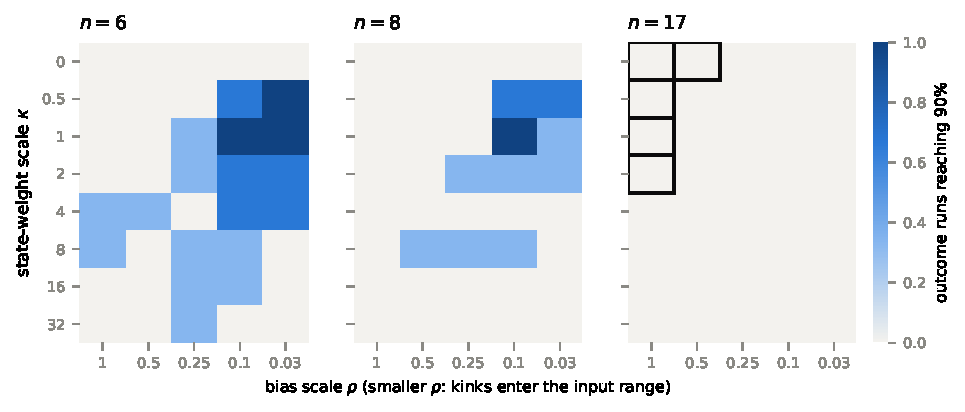
\includegraphics[width=\linewidth]{figures/two_path_sweep.pdf}
\caption{\textbf{Where the outcome trap holds and where it breaks.} Two-path family, zero readout,
three seeds per cell. Cells show the fraction of outcome runs reaching $90\%$ accuracy within $20$k
gradient steps, as the state weights are scaled by $\kappa$ and the biases by $\rho$.
Outlined cells contain seeds that satisfy the outcome certificate. Step training reaches positive
margins in at most $20$ steps in all $360$ runs.}
\label{fig:two-path-sweep}
\end{figure}


\subsection{Joint routing runs}
\label{app:reach}

\Cref{tab:reach} uses the two-block architecture of \cref{app:model}, $K=2,p=1/4$,
full-batch gradient descent of step size $2$, $4{,}096$ training prompts and $16{,}384$
held-out prompts. Fan-in weights, embeddings of variance $1/d_{\mathrm{res}}$ and
MLP biases of magnitude $1$--$2$ are scaled by $\varepsilon=0.3$; readout and relative
biases start at zero. Only QK, relative biases and readout train. Success means every
held-out state has positive margin. The remaining $n=12$ run reaches $99.95\%$ by
$300$k updates; matched outcome runs solve none. Per-run measurements are in the repository.

%=============================================================================
\section{Reproducibility}
\label{app:reproducibility}

% TODO before submission: confirm the anonymous repository URL.
\paragraph{Code.} \url{https://anonymous.4open.science/r/trace} provides exact executors,
configurations, seeds, reproduction commands, per-run measurements and numerical checks
of credit, plateau, reduced two-path executor and attracting-minimum claims.

\paragraph{Compute and data.} One NVIDIA A100 80GB GPU takes about one minute per $8$k
counting updates; the two-path runs use CPU only. Exploratory compute was additional. All data are synthetic.
Software: PyTorch 2.13 (BSD-3-Clause), NumPy and SciPy (BSD-3-Clause).
